\subsection{Acquisition outcome ledger}

The continuation attempted 1 new public YouTube watch request and 1 independent author-transcript request. Successful new operations: 0; new caption documents: 0; new media downloads: 0. The corpus index holds 925 inherited upload metadata records and 0 newly indexed transcript artifacts. The author HTTP 403 and YouTube proxy CONNECT 403 are distinct observations; neither means that a source does not exist.

\subsection{Retained descriptive checks}

Earlier descriptive findings remain available with their original definitions. The caption pilot is shorter in median duration than the nonpilot known-duration pool; title-keyword duration contrasts change with per-account weighting; the former 22-video/eleven-account centroid comparison is distinct from the new 25-video upload-pair diagnostic. They provide context rather than independent replication of the continuation analyses.

\begin{figure*}[t]
\centering
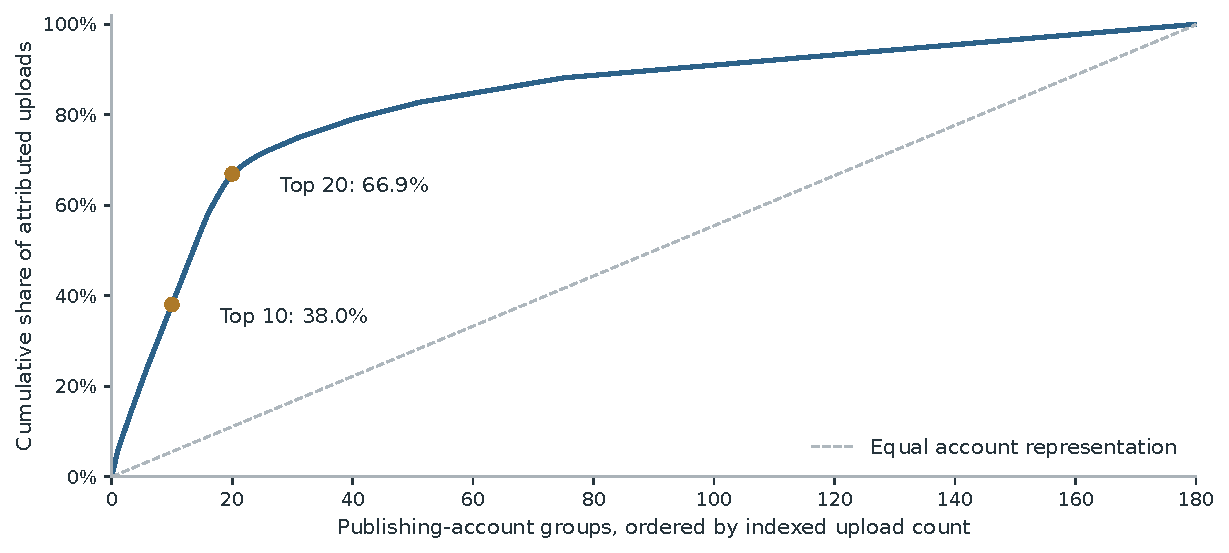
\includegraphics[width=\textwidth]{generated/figures/retained-concentration.pdf}
\caption{Retained publisher concentration among attributed indexed uploads, not population prevalence.}
\label{fig:retained-concentration}
\end{figure*}

\begin{figure*}[t]
\centering
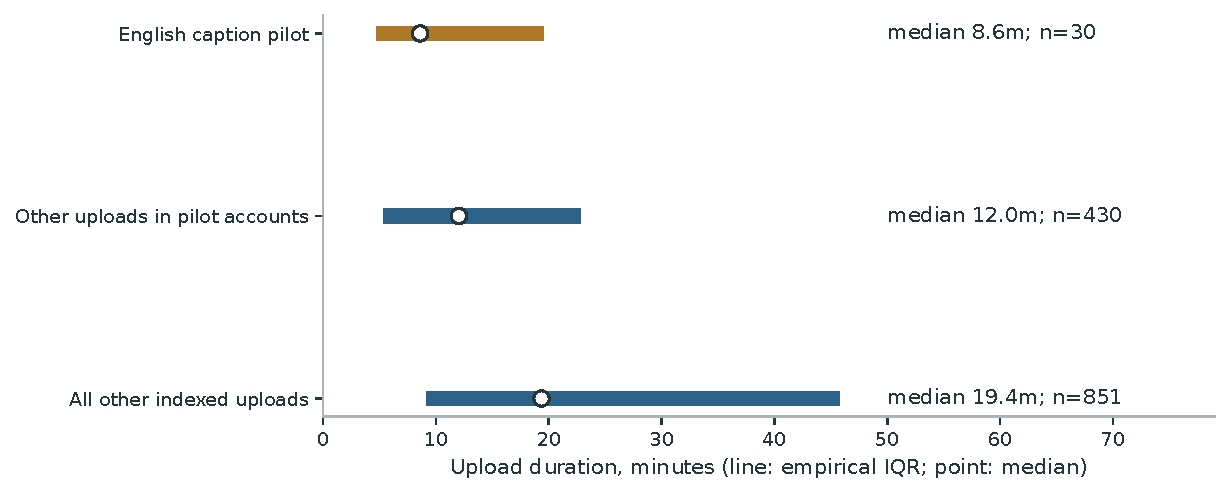
\includegraphics[width=\textwidth]{generated/figures/retained-caption-selection.pdf}
\caption{Retained selected-caption duration comparison. Interquartile spans are empirical distributions, not confidence intervals.}
\label{fig:retained-caption-selection}
\end{figure*}

\begin{figure*}[t]
\centering
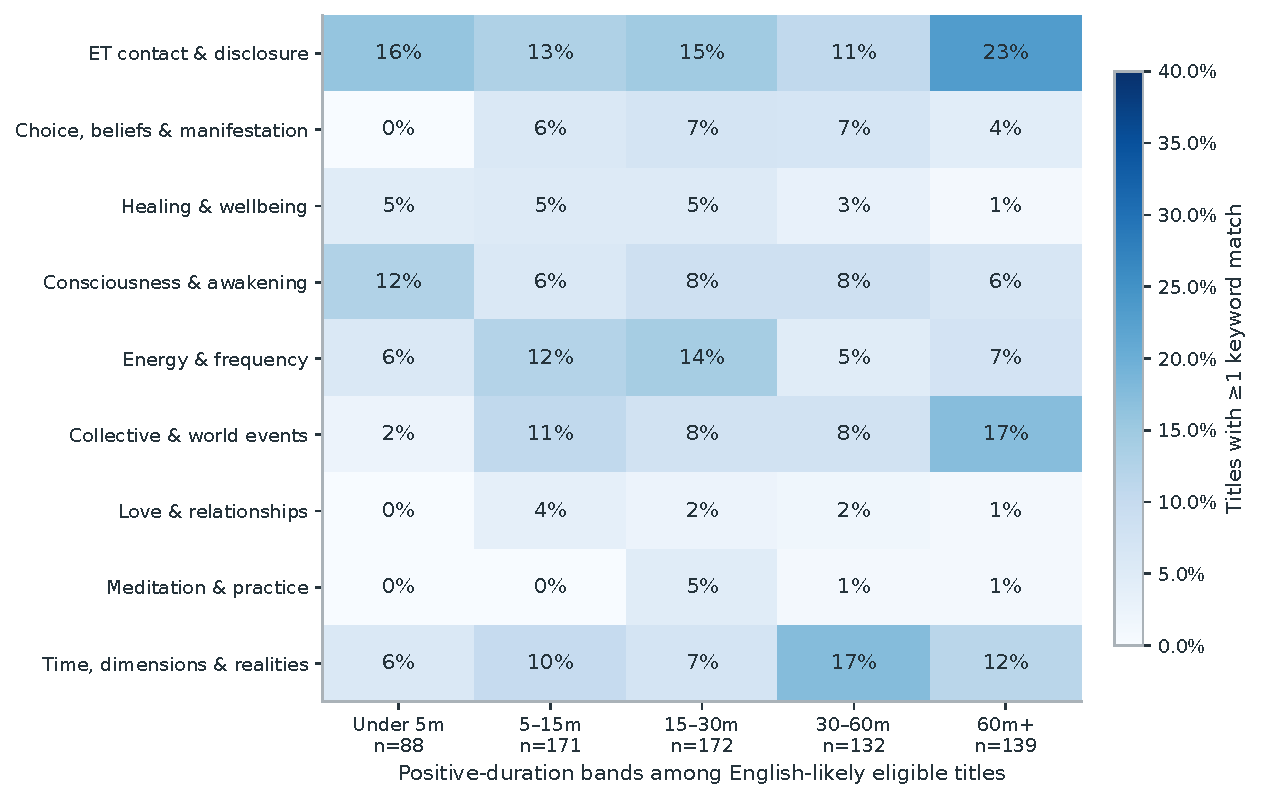
\includegraphics[width=\textwidth]{generated/figures/retained-keyword-duration.pdf}
\caption{Retained title keyword presence by measured duration. The 702 eligible titled uploads with known duration define the denominator; overlapping dictionary families are unvalidated indicators.}
\label{fig:retained-keyword-duration}
\end{figure*}

\subsection{Lexical source-family rule sensitivity}

The stricter proxy requires repeated question-pair links at each listed cosine threshold. Its group counts describe that alternative rule, rather than the more inclusive guard used to split the local-model pilot. Neither rule verifies original-session identity.

\begin{table}[t]
\centering\small\setlength{\tabcolsep}{3pt}
\begin{tabular}{p{0.23\columnwidth}p{0.23\columnwidth}p{0.23\columnwidth}p{0.2\columnwidth}}
\toprule
Min cosine & Links needed & Upload links & Groups \\ \midrule
0.70 & 2 & 6 & 62 \\
0.80 & 2 & 4 & 64 \\
0.90 & 2 & 4 & 64 \\
\bottomrule
\end{tabular}
\caption{Stricter repeated-question-pair source proxy. This rule differs from the more inclusive benchmark guard and must not be described as the same session classification.}
\end{table}

\subsection{Model-assisted reading artifacts}

The retained repository files \path{research/expansion/qa/close-reading.json} and \path{research/expansion/qa/pair-close-reading.json} contain twenty single-candidate and twelve paired model-assisted readings, respectively. Each links to digest source pointers and hashes. The inspected material is the existing AI-generated question and gist fields; no human annotation, raw transcript, audio or video inspection is claimed by these ledgers. All paired answer-agreement fields remain undetermined.

One paired reading identifies compatible life-purpose paraphrases despite different answer wording; another retains uncertainty about relative versus calendar contact windows because original recording dates are unresolved. These interpretations illustrate why a lexical score alone cannot establish contradiction or chronological drift. They are selected interpretive examples, not a representative validation sample.
